\chapter{Wat is de huidige staat van de Appsemble UX}
\section{Bankai UX Review}
Om er achter te komen wat de staat Appsemble UX is het van belang dat we weten wat de zwakke punten zijn. Om hierachter te komen zijn we gaan zitten met een UX gespecialiseerd bedrijf, \href{http://www.bankai.eu/}{Bankai}\cite{bankai}.\\
\newline
%
Aan de hand van de hand van de feedback van Bankai is een goed beeld te krijgen waar nog niet gerealiseerde potentie ligt, de resultaten hiervan staan hieronder beschreven met screenshots ter verduidelijking.\\
\newline
%
De Appsemble homepage mist op dit moment een appeal, iets waarop een klant kan zien wat er met Appsemble te maken is, iets waar ze enthousiast van worden om het te gaan gebruiken. Momenteel ziet het geheel er niet erg aantrekkelijk uit en er mist een duidelijke call to action.\\
\newline
\begin{figure}[H]
	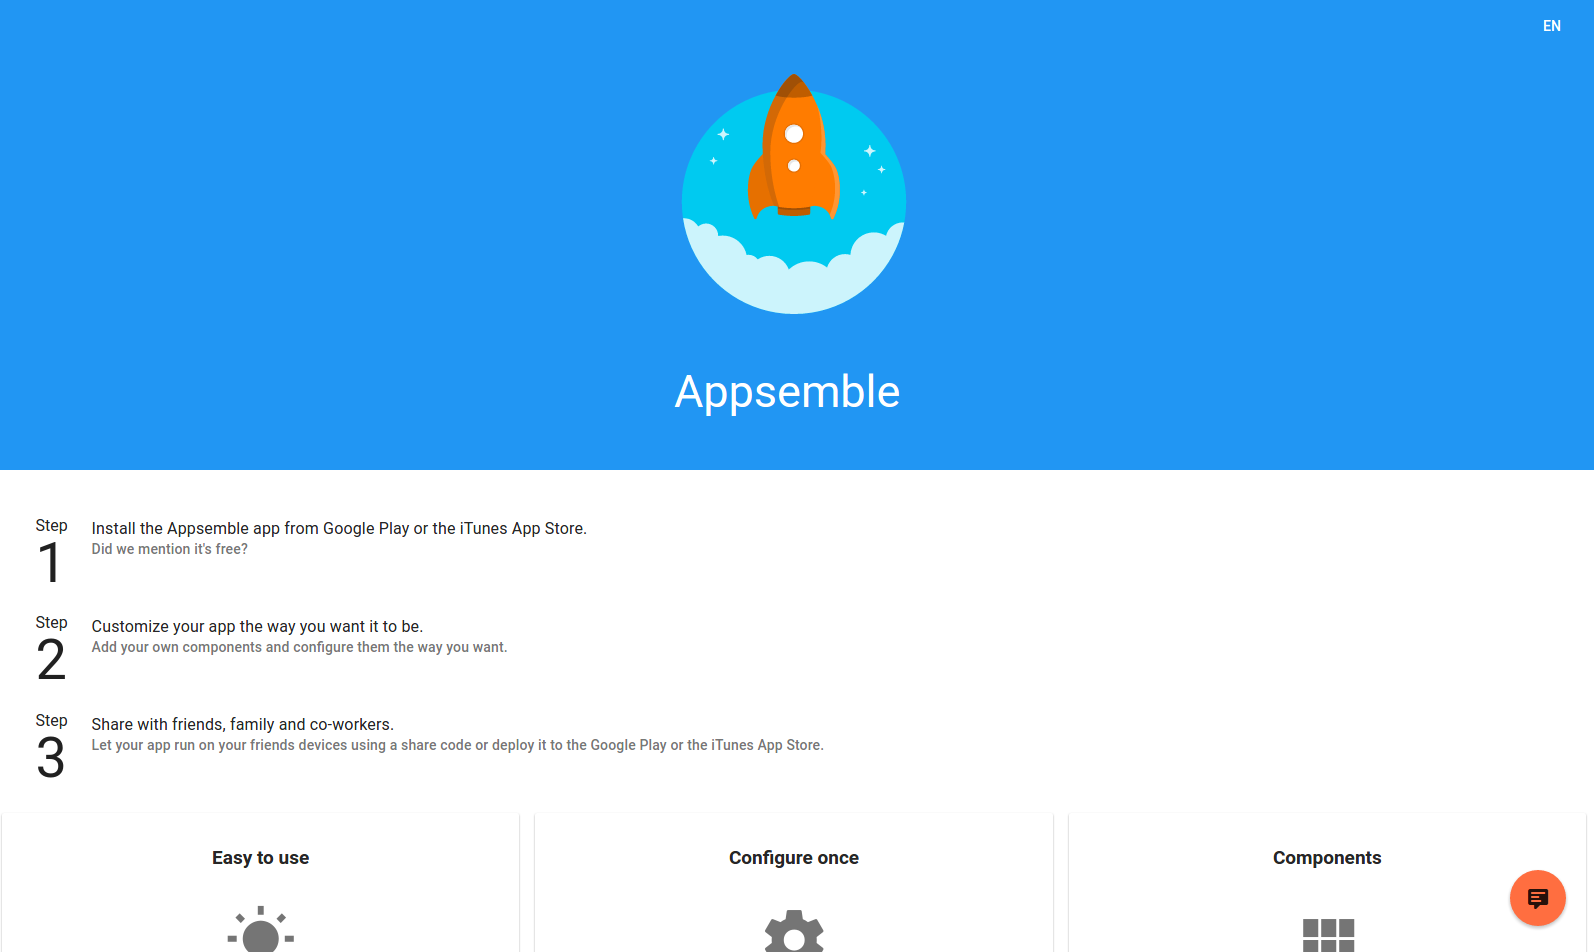
\includegraphics[width=\linewidth]{images/appsemble_landing_page}
	\caption{Appsemble landing page}
\end{figure}
Dit is de huidige landing page van Appsemble, de meerderheid van de pagina bestaat uit lege ruimte. Wat er wel op de pagina staat zijn een aantal stappen voor het maken van een app met Appsemble, deze stappen zijn echter niet de selling points van Appsemble, deze staan onder de fold (de gebruiker moet naar beneden scrollen om te deze te zien). Deze pagina mist ook een Call to Action, de gebruiker moet op Build drukken in de sidebar om te beginnen (dit staat ook nergens uitgelegd en moet de gebruiker zelf uitvinden).  Een voorbeeld van een intro tekst blok is te vinden op de tutorial pagina, deze tekst zou beter op de landing page passen.\\
\newline
\begin{figure}[H]
	\centering
	
\includegraphics[scale=0.25]{images/appsemble_start_page}
	\caption{Appsemble start page}
\end{figure}
Zodra de gebruiker daadwerkelijk zijn app wil gaan bouwen komt hij op een scherm waar hij kan kiezen om een nieuwe app te maken of in te loggen, dit scherm lijkt  echter de optie te missen om een app te laden. De login knop bied deze functie echter wel maar de naam doet vermoeden dat je alleen maar met de knop inlogt.\\
\newline
\begin{figure}[H]
	\centering
	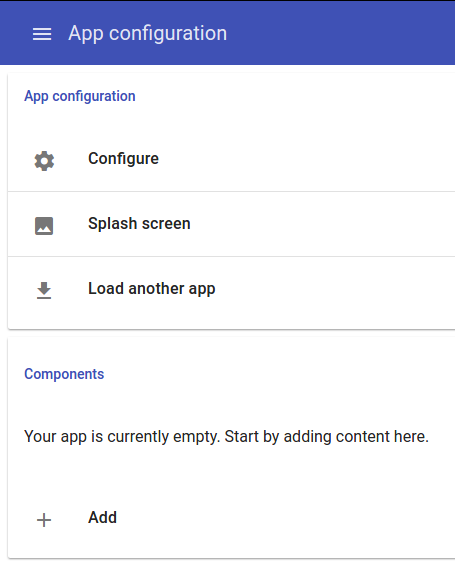
\includegraphics[scale=0.3]{images/appsemble_configuration_page}
	\caption{Appsemble configuration page}
\end{figure}
Zodra de gebruiker op create new app heeft geklikt komt hij in dit scherm terecht. Dit scherm is voor veel gebruikers niet wat ze verwachten te zien.Op de pagina staan verschillende onderdelen met complexe termen als configureren en componets, dit kunnen struikelblokken zijn voor een gebruiker en maken het geheel erg verwarrend en complex voor een gebruiker.\\
\newline
\begin{figure}[H]
	\centering
	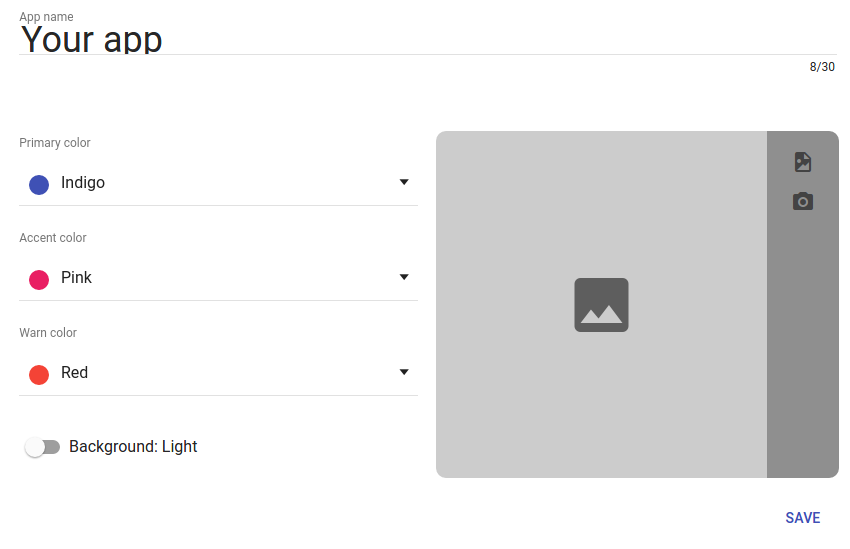
\includegraphics[scale=0.3]{images/appsemble_configure_page}
	\caption{Appsemble configuration page}
\end{figure}
Als de gebruiker op de configure knop drukt kan hij een aantal eigenschappen van zijn app 
aanpassen zoals het kleuren schema en kan hij een icoontje voor zijn app kiezen.\\
\newline
Voor iemand die niet gewend is om dingen als een naam, een kleuren thema \& een icon te kiezen kan dit afschrikkend werken. Door een gebruiker hier hulp in te bieden zou de drempel om een app te publiceren lager zijn. \\
\newline
Door de applicatie worden complexe termen gebruikt zoals Metadata \& Build, dit kan een afschrikkende werking hebben voor gebruikers, het zou beter zijn om deze termen te veranderen in bijvoorbeeld app informatie \& publish.\\
\newline
De app mist verder een duidelijke flow die de gebruiker door de applicatie heen leidt, hierdoor raken gebruikers verdwaald, verward of gefrustreerd. De oplossing hiervoor zou zijn om een duidelijk flow neer te zetten zodat de gebruiker niet hoeft na te denken over hoe hij iets moet doen maar het instinctief weet.\\
\newline
Verder is er geen sprake van onboarding binnen het platform, er zijn tutorials beschikbaar maar deze gaan niet heel erg in detail en de informatie die er staat zou ook tijdens een onboarding kunnen worden behandeld.\\
\section{Job Shadowing}
Om een indruk te krijgen van hoe de gemiddelde gebruiker met Appsemble werkt is er een Job Shadowing uitgevoerd, in deze sessie word de website aan de gebruiker gepresenteerd en krijgt deze een opdracht om een bepaalde taak uit te voeren. Er wordt vastgelegd wat de gebruiker doet en de gebruiker wordt gevraagd om hardop na te denken.\\
\newline
Iedere gebruiker krijgt de volgende opdrachten:
\begin{enumerate}
	\item Maak een nieuwe app aan.
	\item Voeg 2 onderdelen toe aan de app.
	\item Verwijder een onderdeel van de app.
	\item Verberg een onderdeel van de app.
	\item Geef de app een titel en een eigen stijl
	\item Publiceer je app op de Google Play Store en de App Store
\end{enumerate}
De applicatie zal door meerdere soorten gebruikers getest worden om een zo duidelijk mogelijk beeld te krijgen van de huidige staat van de Appsemble UX.
\subsection{IT-Professional}
\subsection{Tech savvy gebruiker}
\subsection{Literally my grandma}
